\documentclass{experimento}

\begin{document}

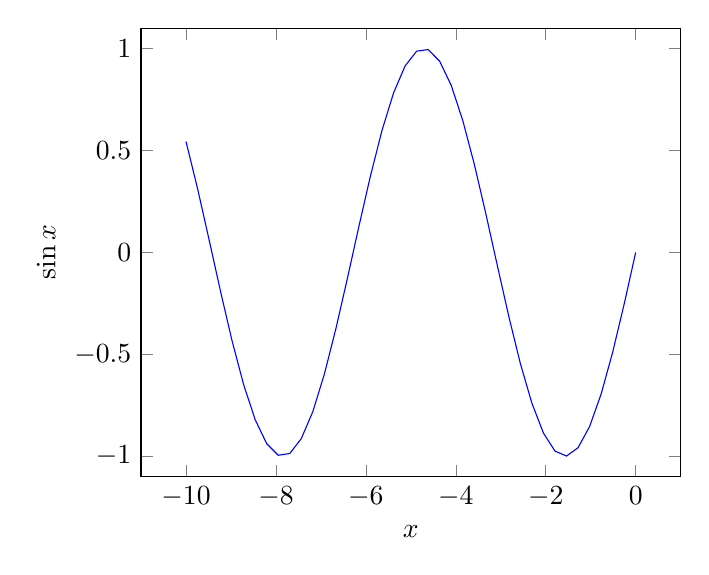
\begin{tikzpicture}
  \begin{axis}[
  ymax=1.1, ymin=-1.1,
  xlabel=$x$,ylabel=$\sin x$,
  ]
  \addplot [
  blue,mark=none,
  domain=-10:0,samples=40,
  ] {sin(deg(x))};
  \end{axis}
\end{tikzpicture} \par

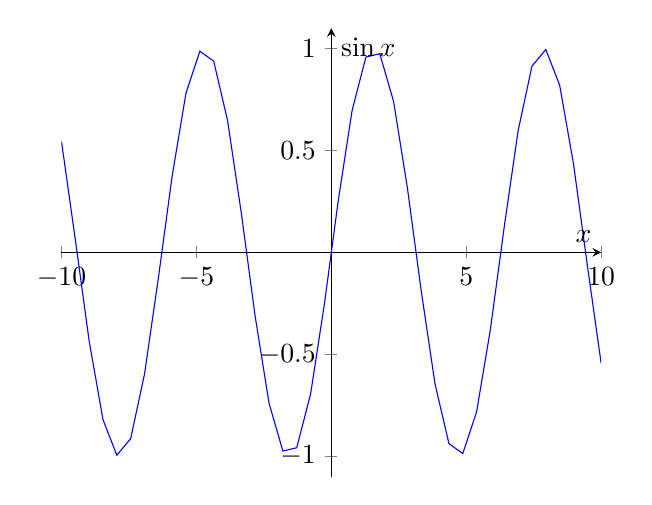
\begin{tikzpicture}
  \begin{axis}[
  axis y line=center,
  axis x line=middle,
  ymax=1.1, ymin=-1.1,
  xlabel=$x$,ylabel=$\sin x$,
  ]
  \addplot [
  blue,mark=none,
  domain=-10:10,samples=40,
  ] {sin(deg(x))};
  \end{axis}
\end{tikzpicture} \par



\begin{tikzpicture}
  \begin{axis}[
  axis y line=center,
  axis x line=middle,
  xlabel=$x$,ylabel=$y$,
  axis line style={-{Triangle[round]},shorten >=-10pt},
  xlabel style={
    at={(xticklabel* cs:1.05)},
    anchor=west,
  },
  ylabel style={
    at={(yticklabel* cs:1.06)},
    anchor=south,
  },
  %enlarge x limits={upper, value=0.1},  % Extends x-axis by 10% beyond xmax
  %enlarge y limits={upper, value=0.1},  % Extends y-axis by 10% beyond ymax
  axis on top,  % Ensures axis lines are drawn on top of the grid
  ]
  
  \addplot [
  smooth,blue,mark=none,
  domain=-5:0,samples=40,
  ] {sin(deg(x))};
  \end{axis}
  \end{tikzpicture}

\pgfplotsset{
  eje escolar/.style={
    axis y line=center,
    axis x line=middle,
    xlabel=$x$,ylabel=$y$,
    axis line style={-{Triangle[round]},shorten >=-10pt},
    xlabel style={
      at={(xticklabel* cs:1.05)},
      anchor=west,
    },
    ylabel style={
      at={(yticklabel* cs:1.06)},
      anchor=south,
    },
    enlargelimits=0.01,  % Extends y-axis by 10% beyond ymax
    axis on top,
    tick label style={
      fill=white,
      fill opacity=0.9,
      inner xsep=1pt,
      inner ysep=1pt,
    },
  }
}

\begin{tikzpicture}
  \begin{axis}[eje escolar, ytick={-1,0,1},
    extra tick style={grid=major}]

    \addplot+[domain=0:5,no marks,smooth,samples=200] {sin(deg(x))};
  \end{axis}
\end{tikzpicture}

\begin{tikzpicture}
  \begin{axis}[eje escolar, ytick={-1,1},
    extra tick style={grid=major},xtick={pi/2,pi,3*pi/2,2*pi},
    xticklabels={$\dfrac{\pi}{2}$,$\pi$,$\dfrac{3\pi}{2}$,$2\pi$}]
    \addplot+[domain=0:2*pi,no marks,smooth,samples=100] {sin(deg(x))} 
      node[pos=0.4,pin={[pin edge={Triangle[round]-}]above right:Seno}] {};
  \end{axis}
\end{tikzpicture}

\tikzset{
    every pin/.style={pin edge={Triangle[]-}},
}

\begin{tikzpicture}
  \begin{axis}[eje escolar,
    ytick={-1,1},
    extra tick style={grid=major},xtick={pi/2,pi,3*pi/2,2*pi},
    xticklabels={$\dfrac{\pi}{2}$,$\pi$,$\dfrac{3\pi}{2}$,$2\pi$}]
    \addplot+[domain=0:2*pi,no marks,smooth,samples=100] {sin(deg(x))} 
      node[pos=0.4,pin=above right:Seno] {};

    \addplot+[domain=0:2*pi,no marks,smooth] {cos(deg(x))}
      node[pos=0.4,pin=left:Coseno] {};

  \end{axis}
\end{tikzpicture}


\begin{tikzpicture}
  \begin{axis}[eje escolar,cycle list name=linestyles,
    ytick={-1,1},
    extra tick style={grid=major},xtick={pi/2,pi,3*pi/2,2*pi},
    xticklabels={$\dfrac{\pi}{2}$,$\pi$,$\dfrac{3\pi}{2}$,$2\pi$},smooth,
    trig format plots=rad,
    legend style={
      at={(1.05,1)},
      anchor=north west,
      cells={anchor=west},
      font=\footnotesize,
      nodes={
        inner xsep=0.1em,  % Reduce horizontal spacing between symbol and text
        inner ysep=0.1em,  % Reduce vertical spacing between legend entries
      }
    }
    ]
    \addplot[domain=0:2*pi] {sin(x)};
    \addplot[domain=0:2*pi,dashed] {cos(x)};
    \addplot[domain=0:2*pi,update limits=false,
      restrict y to domain=-10:10,dotted] {tan(x))};
    \legend{Seno,Coseno,Tangente};

  \end{axis}
\end{tikzpicture}

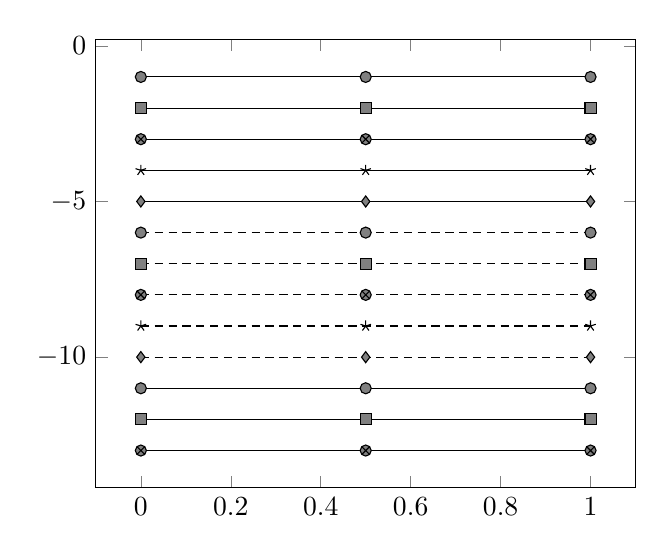
\begin{tikzpicture}
  \begin{axis}[
  stack plots=y,stack dir=minus,
  cycle list name=black white]
  \addplot coordinates {(0,1) (0.5,1) (1,1)};
  \addplot coordinates {(0,1) (0.5,1) (1,1)};
  \addplot coordinates {(0,1) (0.5,1) (1,1)};
  \addplot coordinates {(0,1) (0.5,1) (1,1)};
  \addplot coordinates {(0,1) (0.5,1) (1,1)};
  \addplot coordinates {(0,1) (0.5,1) (1,1)};
  \addplot coordinates {(0,1) (0.5,1) (1,1)};
  \addplot coordinates {(0,1) (0.5,1) (1,1)};
  \addplot coordinates {(0,1) (0.5,1) (1,1)};
  \addplot coordinates {(0,1) (0.5,1) (1,1)};
  \addplot coordinates {(0,1) (0.5,1) (1,1)};
  \addplot coordinates {(0,1) (0.5,1) (1,1)};
  \addplot coordinates {(0,1) (0.5,1) (1,1)};
  \end{axis}
\end{tikzpicture}

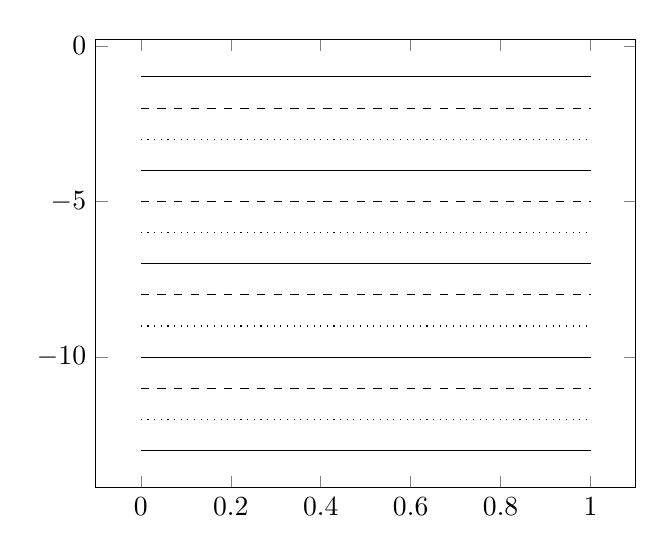
\begin{tikzpicture}
  \begin{axis}[
  stack plots=y,stack dir=minus,
  cycle list name=linestyles,]
  \addplot coordinates {(0,1) (0.5,1) (1,1)};
  \addplot coordinates {(0,1) (0.5,1) (1,1)};
  \addplot coordinates {(0,1) (0.5,1) (1,1)};
  \addplot coordinates {(0,1) (0.5,1) (1,1)};
  \addplot coordinates {(0,1) (0.5,1) (1,1)};
  \addplot coordinates {(0,1) (0.5,1) (1,1)};
  \addplot coordinates {(0,1) (0.5,1) (1,1)};
  \addplot coordinates {(0,1) (0.5,1) (1,1)};
  \addplot coordinates {(0,1) (0.5,1) (1,1)};
  \addplot coordinates {(0,1) (0.5,1) (1,1)};
  \addplot coordinates {(0,1) (0.5,1) (1,1)};
  \addplot coordinates {(0,1) (0.5,1) (1,1)};
  \addplot coordinates {(0,1) (0.5,1) (1,1)};
  \end{axis}
  \end{tikzpicture}

\end{document}